\documentclass[10pt,twocolumn,letterpaper]{article}

% =====================================================================
% CVPR/ICCV submission template (draft-standalone preamble).
% Swap for \usepackage[review]{cvpr} + the official cvpr.sty when packaging.
% =====================================================================

\usepackage[margin=0.9in]{geometry}
% \usepackage{times}  % enable with official template (needs courier TFM)
\usepackage{graphicx}
\usepackage{amsmath,amssymb}
\usepackage{booktabs}
\usepackage{multirow}
\usepackage{xcolor}
\usepackage[colorlinks=true,allcolors=blue]{hyperref}
\usepackage{caption}

\graphicspath{{figs/}}
\renewcommand{\ttdefault}{cmtt}   % draft-only monospace fallback

\title{Learning Disocclusion Reliability:\\ When and Where a Generative Prior Helps Single-View Reconstruction}
\author{Anonymous submission\\\small Paper ID ****}
\date{}

\begin{document}
\maketitle

\begin{abstract}
Single-view 3D reconstruction systems fail unevenly: some disoccluded regions
can be reconstructed by a feed-forward model, while others require generative
completion. We study the reliability prediction problem: before invoking a slow
generative teacher, can we predict whether it will help --- and where? We
formulate disocclusion reliability learning as predicting teacher usefulness
from test-time observable features. At the \emph{scene} level the problem is
data-limited: a simple visible-gap rule is already a strong policy and a learned
scene-level ReliabilityNet only matches it (N=166 scenes: rule $+0.87$ dB vs
learned $+1.13$ dB, both below oracle $+1.70$ dB). The key result is that moving
to the \emph{frame} level unlocks learning: with 2{,}898 frame-level samples a
logistic frame ReliabilityNet reaches \textbf{0.87 accuracy, ROC-AUC 0.95,
PR-AUC 0.96}, and \textbf{$+1.60$ dB mean invisible-PSNR gain --- 94\% of the
oracle's $+1.70$ dB --- clearly beating the visible-gap rule ($+0.89$ dB) while
saving 41\% of teacher calls}. A tunable risk-averse operating point drives the
worst case toward zero while remaining net-positive. Descending further to the
\emph{patch} level, prediction becomes hard (ROC-AUC 0.72) and the gain over
always-injecting nearly vanishes, identifying the frame as the sweet spot.
Across granularities the governing mechanism is stable: the correlation between
the geometry-expert-vs-baseline invisible gap and the actual teacher improvement
is $+0.98$.
\end{abstract}

\section{Introduction}
\label{sec:intro}
A generative disocclusion prior (e.g. a diffusion backbone guided by a
feed-forward geometry expert) can substantially improve novel-view quality in
disoccluded regions, but it is expensive and \emph{not uniformly beneficial}: on
scenes where the feed-forward baseline already reconstructs the invisible region
well, invoking the generative teacher hurts. This makes reliability prediction a
first-class problem: we want to call the teacher only when, and ideally only
where, it will help.

We formulate this as supervised reliability learning from test-time observable
features (the geometry expert's self-metrics, camera motion, disocclusion
statistics), with labels given by whether the teacher actually reduces
invisible-region error. Our study answers three questions: (i) is scene-level
reliability learnable? (ii) does finer granularity help? (iii) is there a lower
bound on useful granularity? We find that the frame level is the sweet spot: it
provides enough samples for a learned predictor to beat a strong rule and
approach the oracle, while exposing a tunable mean-vs-worst-case frontier.

\paragraph{Contributions.}
\begin{enumerate}
\item We formulate disocclusion reliability as a learnable scheduling problem
with purely test-time-observable features and teacher-usefulness labels.
\item We show a granularity effect: scene-level is data-limited (learned $\approx$
rule), frame-level unlocks learning (ROC-AUC 0.95, 94\% of oracle, 41\% compute
saved), and patch-level is hard (ROC-AUC 0.72), so the frame is the sweet spot.
\item We expose a tunable mean-vs-worst-case operating frontier and a stable
$+0.98$ governing mechanism reproduced across scales.
\end{enumerate}

\section{Related Work}
\label{sec:related}
Our predictor is a form of test-time routing / cascade: decide from cheap
observable signals whether to invoke an expensive expert. This is related to
model cascades and deferral, but instantiated for single-view 3D disocclusion,
where the ``expert'' is a generative prior~\cite{viewcrafter,cat3d,genwarp} over
a feed-forward reconstructor~\cite{flash3d,pixelsplat,mvsplat,depthsplat}. The
governing signal we exploit --- the invisible-region gap between the geometry
expert and the generative baseline --- is the same mechanism identified for
selective test-time injection in the companion paper, here turned into a learned,
deployable scheduler.

\section{Method}
\label{sec:method}
\paragraph{Problem.} For each unit (scene / frame / patch) we predict a binary
label: will the generative teacher reduce invisible-region MSE relative to the
feed-forward baseline? Features are test-time observable: the geometry expert's
visible/invisible self-PSNR, the visible gap (expert visible $-$ baseline
visible), disocclusion fraction, and --- at frame level --- camera translation
and rotation from the source view plus interaction terms.

\paragraph{Predictor.} A logistic ReliabilityNet is trained under grouped
leave-one-scene-out cross-validation so that no frames/patches from a test scene
appear in training (no leakage). At test time a threshold on the predicted
probability decides whether to invoke the teacher, tracing a mean-vs-worst-case
operating frontier.

\section{Experiments}
\label{sec:exp}

\subsection{Scene-level: the problem is data-limited (N=166)}
\begin{table}[t]
\centering\small
\caption{Scene-level policies (N=166, LOOCV). Learned only slightly edges the
rule; scene features saturate.}
\begin{tabular}{lrrr}
\toprule
Policy & Mean $\Delta$ & Worst & Inject \\
\midrule
Always teacher & $+0.75$ & $-11.72$ & 166/166 \\
Rule \texttt{vis\_gap$>$0} & $+0.87$ & $-8.51$ & 162/166 \\
Scene ReliabilityNet (LOOCV) & $+1.13$ & $-6.80$ & 114/166 \\
Oracle & $\mathbf{+1.70}$ & $0.00$ & 98/166 \\
\bottomrule
\end{tabular}
\end{table}
The learned net's margin over the rule grows monotonically with data (parity at
N=92; $+0.11$ at N=129; $+0.19$ at N=149; $+0.26$ at N=166), indicating the
scene level is data-limited rather than unlearnable.

\subsection{Frame-level: learning unlocks the gain (2{,}898 frames, 74 scenes)}
\begin{table}[t]
\centering\small
\caption{Frame-level policies (2{,}898 frames, grouped-CV). The learned predictor
beats the rule by a wide margin and reaches 94\% of the oracle while saving 41\%
of teacher calls.}
\begin{tabular}{lrrrr}
\toprule
Policy & Mean $\Delta$ & Worst & ROC-AUC & Saved \\
\midrule
Always teacher & $+0.48$ & $-23.09$ & --- & 0\% \\
Rule \texttt{vis\_gap$>$0} & $+0.89$ & $-10.63$ & --- & 14\% \\
Frame ReliabilityNet & $\mathbf{+1.60}$ & $-2.61$ & $\mathbf{0.949}$ & 41\% \\
Oracle & $+1.70$ & $0.00$ & --- & 43\% \\
\bottomrule
\end{tabular}
\end{table}
The frame ReliabilityNet reaches accuracy 0.87, ROC-AUC 0.949, PR-AUC 0.958
(0.961 with camera-motion features). As the pool grows to 2{,}898 frames the
newly added scenes have lower average teacher gain (always-inject drops to
$+0.48$ dB), yet the learned predictor still recovers $+1.60$ dB --- the harder
the pool, the more selective scheduling matters. Figures~\ref{fig:frontier},
\ref{fig:rocpr}, \ref{fig:saved} show the operating frontier, ROC/PR curves, and
compute-vs-quality trade-off.

\begin{figure}[t]
\centering
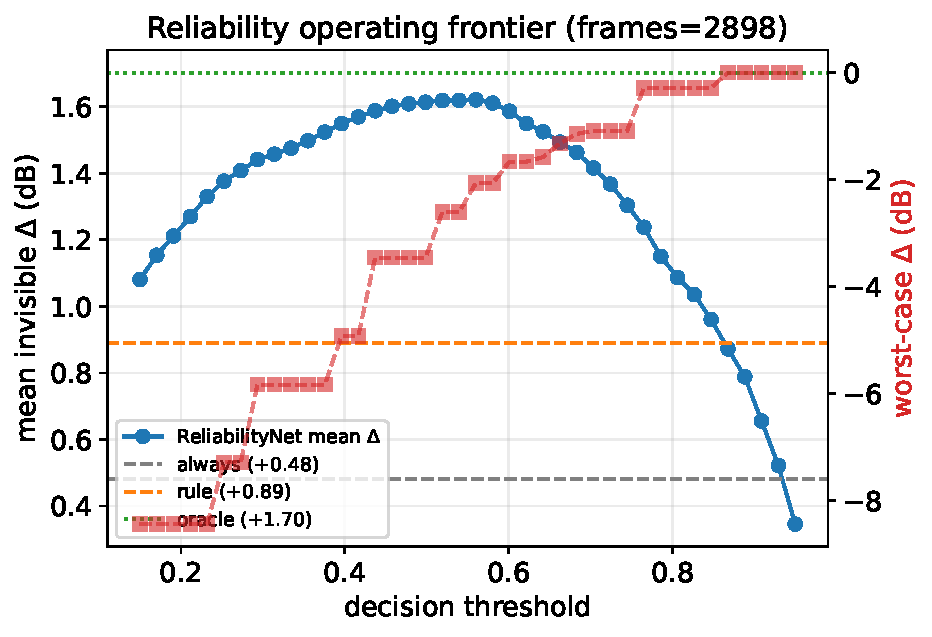
\includegraphics[width=\linewidth]{fig4_frontier.pdf}
\caption{Mean-vs-worst-case operating frontier as the decision threshold varies.
A fixed rule is a single point; the learned predictor spans a frontier, letting
an operator choose maximum quality or near-zero-risk operation.}
\label{fig:frontier}
\end{figure}

\begin{figure}[t]
\centering
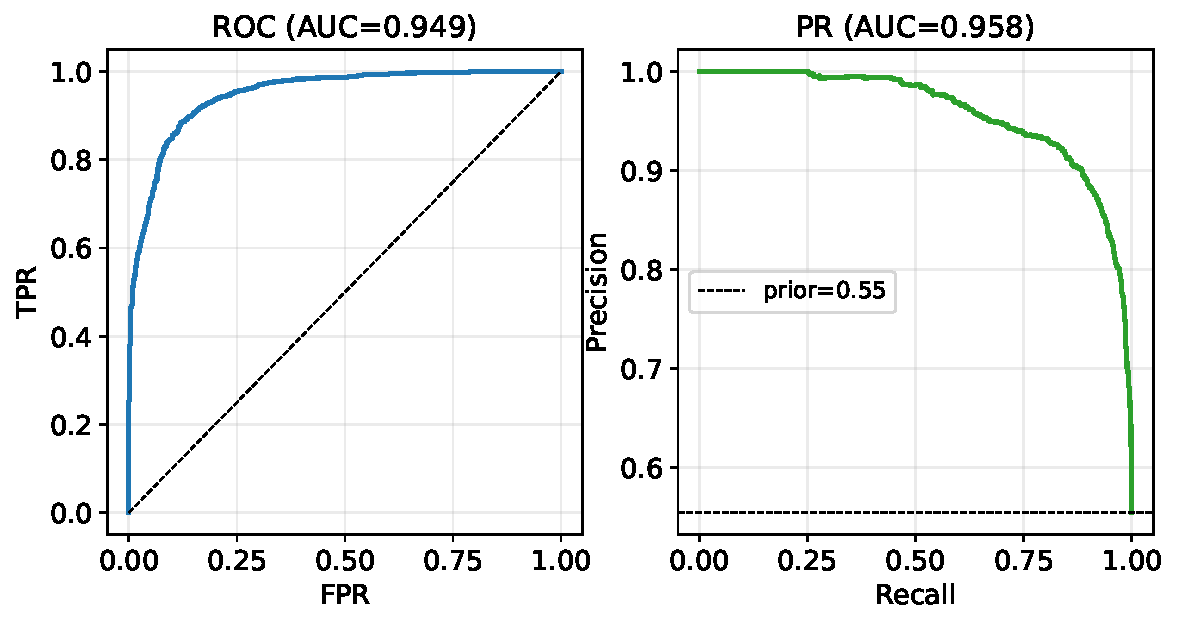
\includegraphics[width=\linewidth]{fig5_roc_pr.pdf}
\caption{Frame-level ROC and precision-recall curves (grouped-CV). ROC-AUC 0.95,
PR-AUC 0.96.}
\label{fig:rocpr}
\end{figure}

\begin{figure}[t]
\centering
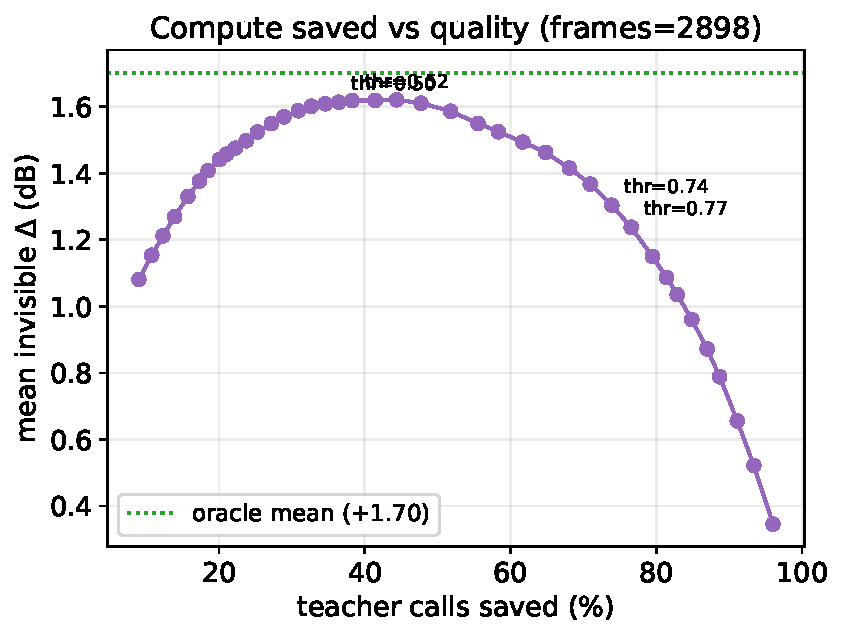
\includegraphics[width=\linewidth]{fig6_saved.pdf}
\caption{Compute saved vs quality retained: the predictor keeps most of the
oracle gain while skipping a large fraction of teacher calls.}
\label{fig:saved}
\end{figure}

\subsection{Patch-level: the granularity has a lower bound}
Using 8$\times$8 patch tiling with only test-time-observable patch features
(geometry-expert-vs-baseline L1 disagreement and its variance, baseline
gradient, disocclusion fraction, patch position, expert activity), patch
reliability is substantially harder to predict (ROC-AUC 0.724 vs 0.95 at frame
level, 13{,}831 patches / 21 scenes) and the learned patch gate barely improves
over always-injecting ($+3.20$ vs $+3.05$ dB, far from the $+4.15$ dB oracle).
On high-gain scenes 71\% of disoccluded patches are already teacher-favorable, so
the within-frame signal is weak. This is an honest negative boundary result: the
frame is the sweet spot --- coarse enough for a strong learnable signal, fine
enough to capture per-view variation the scene level misses.

\subsection{Comparison with Standard Routing Baselines}
Reliability routing is an instance of expert deferral / model cascades. We
compare against standard routing baselines at matched compute budget ($\sim$59\%
teacher-call rate, i.e.\ 41\% saved):

\begin{table}[t]
\centering\small
\caption{Routing-policy comparison at matched budget (59\% calls = 41\% compute
saved). Our learned scheduler beats random, always-call, and top-K observable
ranking at the same cost, reaching 94\% of the oracle.}
\begin{tabular}{lrr}
\toprule
Routing policy & Mean $\Delta$ (dB) & Note \\
\midrule
Random @59\% & $+0.26$ & uninformed \\
Always call & $+0.48$ & 0\% saved \\
Vis-gap top-K @59\% & $+1.08$ & strongest rule \\
\textbf{FrameNet (ours) @59\%} & $\mathbf{+1.60}$ & learned \\
Oracle & $+1.70$ & upper bound \\
\bottomrule
\end{tabular}
\end{table}

\subsection{Stable mechanism across granularities}
The correlation between the observable invisible gap (expert$_{\text{inv}}-$
baseline$_{\text{inv}}$) and the actual teacher improvement is $+0.982$ (scene,
N=166) and $+0.978$ (frame, 2{,}898). The mechanism governing when the
generative prior helps is the same at both scales and highly predictable.

\section{Discussion}
\label{sec:disc}
The arc is: (i) disocclusion reliability is a real supervised problem; (ii) at
the scene level it is data-limited and a visible-gap rule is a strong
interpretable baseline; (iii) descending to the frame level provides the sample
size that lets a learned predictor beat the rule and approach the oracle while
exposing a tunable mean-vs-worst-case frontier; (iv) descending further to the
patch level, prediction becomes hard and the gain over always-inject nearly
vanishes. The frame is the sweet spot. The practical contribution is the
frontier: an operator can pick maximum quality ($+1.60$ dB) or a conservative
near-zero-risk operating point.

\section{Limitations}
\label{sec:limits}
The predictor uses observable proxy features rather than the true (unobservable)
teacher gain; its ceiling is the oracle it approximates (94\% reached). Patch/
pixel-level selection would need richer per-pixel evidence (e.g. depth
uncertainty) to pay off. Scaling the frame set further and integrating the
predictor as a learned scheduler into the generative-injection and distillation
pipelines are natural next steps.

\section{Conclusion}
\label{sec:concl}
We established disocclusion reliability as a learnable scheduling problem and
delivered a working frame-level predictor that reaches ROC-AUC 0.95, recovers
94\% of the oracle gain, and saves 41\% of teacher calls under an honest
grouped-CV protocol, with a stable $+0.98$ governing mechanism reproduced across
scales and a clear granularity sweet spot at the frame level.

{\small
\bibliographystyle{plain}
\bibliography{refs}
}
\end{document}
